\documentclass[11pt]{article}

% ── Packages ──────────────────────────────────────────────────────────────────
\usepackage[margin=1in]{geometry}
\usepackage{amsmath,amssymb}
\usepackage{graphicx}
\usepackage{booktabs}
\usepackage{hyperref}
\usepackage{natbib}
\usepackage{parskip}
\usepackage{microtype}
\usepackage{xcolor}
\usepackage{titlesec}
\usepackage{enumitem}

% ── Colours ───────────────────────────────────────────────────────────────────
\definecolor{zetgreen}{HTML}{1B3A2E}

% ── Section formatting ────────────────────────────────────────────────────────
\setcounter{secnumdepth}{2}
\titleformat{\section}{\large\bfseries\color{zetgreen}}{\thesection.}{0.5em}{}[\titlerule]
\titleformat{\subsection}{\normalsize\bfseries}{\thesubsection}{0.5em}{}

% ── Hyperref ──────────────────────────────────────────────────────────────────
\hypersetup{
  colorlinks=true,
  linkcolor=zetgreen,
  citecolor=zetgreen,
  urlcolor=zetgreen
}

% ── Math shortcuts ────────────────────────────────────────────────────────────
\newcommand{\Fi}{\mathcal{F}_i}
\newcommand{\Fj}{\mathcal{F}_j}

% ─────────────────────────────────────────────────────────────────────────────
\usepackage{placeins}  % \FloatBarrier, to keep Figure 2 inside Section 3.5
\begin{document}

\begin{center}
  {\LARGE\bfseries Point Calibration Does Not Control Type~I Error\\[4pt]
  Across the Composite Null in a\\[4pt]
  Composed Adaptive Bayesian Design}\\[14pt]
  {\large Lu Qian}\\[4pt]
  {\normalsize\itshape Zetyra $\vert$ Evidence in the Wild \quad
  \href{mailto:maggie@zetyra.com}{maggie@zetyra.com}}\\[6pt]
  {\small JSM 2026 \textbullet\ Session: AI, Machine Learning \& Digital Tools
  in Clinical Development \textbullet\ August 3, 2026}
\end{center}
\vspace{4pt}
\hrule
\vspace{8pt}

% ── Abstract ──────────────────────────────────────────────────────────────────
\begin{abstract}
\noindent
Efficacy thresholds for Bayesian monitoring can be calibrated at a single
assumed control rate.  We examined whether such point calibration controls
Type~I error (T1E) across the composite null in a two-arm Phase~II design
combining
historical control borrowing, Bayesian monitoring, sample size re-estimation
(SSR), and response-adaptive randomization (RAR).  Four isolated numerical
checks passed their stated tolerances, although the RAR diagnostic was a
stand-alone calculation; none evaluated T1E away from the calibration anchor.

The full-design threshold was calibrated to $\alpha = 0.025$ at $p_0 = 0.25$
with no time trend.  Holding that threshold fixed, we varied the common
response rate over $p = 0.20$--$0.45$, with $\delta=0$, along the equality
boundary of the superiority null.  Each rejection probability therefore
estimates T1E.  In the independent grid run, estimated T1E was 0.0236 at the
anchor (MCSE 0.0021), 0.0810 at $p=0.30$, 0.1854 at $p=0.36$, and 0.2786 at
$p=0.45$, where the curve was still increasing.  The two largest rates
characterise the shape of the curve rather than plausible control rates for
this indication; over $p=0.27$--$0.36$ estimated T1E ran 0.0380 to 0.1854.  Thus, no calendar trend or
time-model misspecification was required to produce the control failure.

Disabling SSR and RAR while retaining the full-design threshold did not restore
control: the ablation reached 0.2020 at $p=0.45$, and its contrast with the full
design reversed sign across the evaluated range.  Because the ablation was not
separately calibrated, this contrast does not attribute excess error to
individual components.  In a separate trend-active stress analysis, results
were reported as rejection probabilities rather than T1E for the constant-rate
estimand.  The pooled SSR~$\times$~RAR interaction estimate was $-0.0077$ (95\%
simulation interval $[-0.0157,+0.0002]$), providing no evidence of a
directional interaction.

Point calibration did not provide uniform T1E control.  The evaluated grid
demonstrates a control violation but does not locate the supremum; operating
characteristics should therefore be assessed across prespecified
null-generating conditions.
\end{abstract}

\vspace{4pt}\hrule\vspace{10pt}

% ─────────────────────────────────────────────────────────────────────────────
\section{Introduction}

Computational tools are used to specify priors, simulate operating
characteristics and prepare regulatory submissions.  In the workflow examined
here, the checks applied to such a tool are component-level and numerical: the
implemented calculations are examined in isolation.
This paper asks what those checks do and do not establish about the error rate
of the assembled design.  We make no claim about how widespread that workflow
is; the question is what follows from it where it is used.

The FDA's January 2026 draft guidance on the use of Bayesian methodology in
clinical trials \citep{fda_bayesian_2026} is directly relevant.  It recommends
comprehensive simulation over plausible assumptions, including the background
rate of the endpoint and accrual rate; asks sponsors to discuss the handling of
prior--data conflict; and, for designs calibrated to a Type~I error target,
recommends evaluating Type~I error and power.  (It is draft guidance containing
nonbinding recommendations, and we describe it as such throughout.)  These
recommendations bear on a specific practice, and one this paper examines
directly: an efficacy threshold calibrated at a single assumed control rate,
with that single point then treated as evidence of error control.

This paper makes two claims, at two levels.  The primary claim is about
\textbf{robustness}: an efficacy threshold calibrated at one assumed control
rate does not deliver Type~I error control across the composite null.  The
secondary claim is about \textbf{composition}: at the frozen full-design
threshold, the combined SSR/RAR contrast changes sign across the evaluated
null rates, but the factorial interaction estimates are too imprecise to
support a stable interaction claim in either direction.

Both claims are demonstrated by simulation over a grid of common baseline
rates.  We are explicit about what such a grid can and cannot establish: it
exhibits points at which control fails, but it does not locate or estimate the
supremum of the Type~I error over the null.

The case study was developed with Zetyra; the released R/Quarto implementation
is the reproducibility artifact for this paper.  The platform supports the
argument; it is not the argument itself.

% ─────────────────────────────────────────────────────────────────────────────
\section{Background}

\subsection{What Component-Level Checks Establish}

``Validation'' of clinical trial design software is not a term with a single
agreed meaning.  Where it amounts to documenting that design outputs were
computed with a named package, with cross-checks against published values, it
does not establish maximum numerical deviation across the range of design
parameters, does not guarantee reproducibility under stochastic methods, and
does not account for the behaviour of multiple adaptive components operating
jointly.  The FDA January 2026 draft guidance addresses this directly: it recommends
that operating characteristics be evaluated by comprehensive simulation over
plausible assumptions, discusses prior--data conflict explicitly, and
recommends scenarios spanning plausible values of design inputs---including the
background rate of the endpoint---documented reproducibly.  These are nonbinding
recommendations in a draft document.

The case study was developed with Zetyra.  The released R/Quarto source and
seeds provide the code needed to rerun the primary Rule~B analysis (see
Acknowledgements); exact cross-environment numerical identity is not claimed.
Results were produced under R 4.6.1 with RBesT 1.10-0, rstan 2.32.7 and
posterior 1.7.0; the full \texttt{sessionInfo()} is written to the release on
each render.  The versions matter because the historical-control prior is
fitted through RBesT and every operating characteristic reported here
conditions on that fitted mixture, so the render asserts the mixture against a
frozen full-precision reference and stops if it moves.
The public validation repository documents the broader software checks.

\subsection{Composed Adaptive Designs and Marginal Calibration}
\label{sec:composed-defn}

\textbf{Definition.}  A \emph{composed adaptive design} is a design in which two
or more adaptive mechanisms act at different times on overlapping information
from the evolving trial, before the final analysis.  They need not share a
schedule or a view of the data, and in the design studied here they do not.
RAR updates the allocation probability patient by patient from arm-labelled
outcomes, after a ten-patient burn-in.  The SSR rule fires once, at $n=45$, on
pooled counts with the arm labels withheld.  Bayesian monitoring evaluates
arm-labelled data at the scheduled looks $\{30,45,60,90\}$.  What they share is
the accruing trial itself: each rule alters the data the others subsequently
see.

We do not formalise this as a set-theoretic condition on information sets.
Writing $\Fi \cap \Fj \neq \emptyset$ would not distinguish anything: for
sigma-fields the intersection always contains $\emptyset$ and $\Omega$, so the
condition holds trivially for any pair.  Nor is the converse available---
informational independence does not by itself guarantee that error control
survives adaptation.

The relevant observation is weaker and purely negative.  Let $\phi(X)$ denote
the final rejection rule (Bayesian monitoring), and let $A_1(X_t)$, $A_2(X_t)$
denote the adaptation rules---SSR and RAR---which alter sample size or
allocation based on interim data $X_t$ but do not themselves reject $H_0$.
Each is checked in isolation (the blinded nuisance-parameter SSR satisfies
its pooled-input, algebra and bound checks; RAR tracks
$P(\theta_e > \theta_c)$ within tolerance).  The composed decision rule
is $\phi_{\text{comp}}(X) = \phi\!\bigl(X;\, A_1(X_t),\, A_2(X_t)\bigr)$: the
final rejection indicator evaluated on data whose sample size and allocation
were shaped by the adaptation rules.  The workflow examined here calibrates that
composed rule at a single point, choosing $\gamma^*$ so that
$P_{p_0,\,\delta=0}\!\bigl(\phi_{\text{comp}}(X) = 1\bigr) \approx \alpha$ at
one anchor rate with no trend.  That targets the error rate at that point but
places no bound on
$P_{p,\,\delta}\!\bigl(\phi_{\text{comp}}(X) = 1\bigr)$ for other $(p, \delta)$
in the null.  The component numerical checks add no such bound either, since
none of them evaluates an error rate.

\textbf{Point calibration alone does not establish range control.  Checking
components in isolation, and calibrating the composed rule at a single null
point, places no uniform bound on the error rate of the composed rule over the
null.}  The claim is about a bound, not about every point: continuity in $p$
may constrain the error rate in a neighbourhood of the anchor, and the grid
below shows it does---0.0236 at $p=0.25$ against 0.0380 at $p=0.27$.  Nothing
in the workflow constrains it away from one.  This is a statement about what
those checks fail to establish, not a condition under which inflation must
occur.
Whether it occurs, in which direction and by how much are empirical questions,
which is why the remainder of the paper is a simulation study.
Figure~\ref{fig:composed} illustrates the structure.




\begin{figure}[!t]
  \centering
  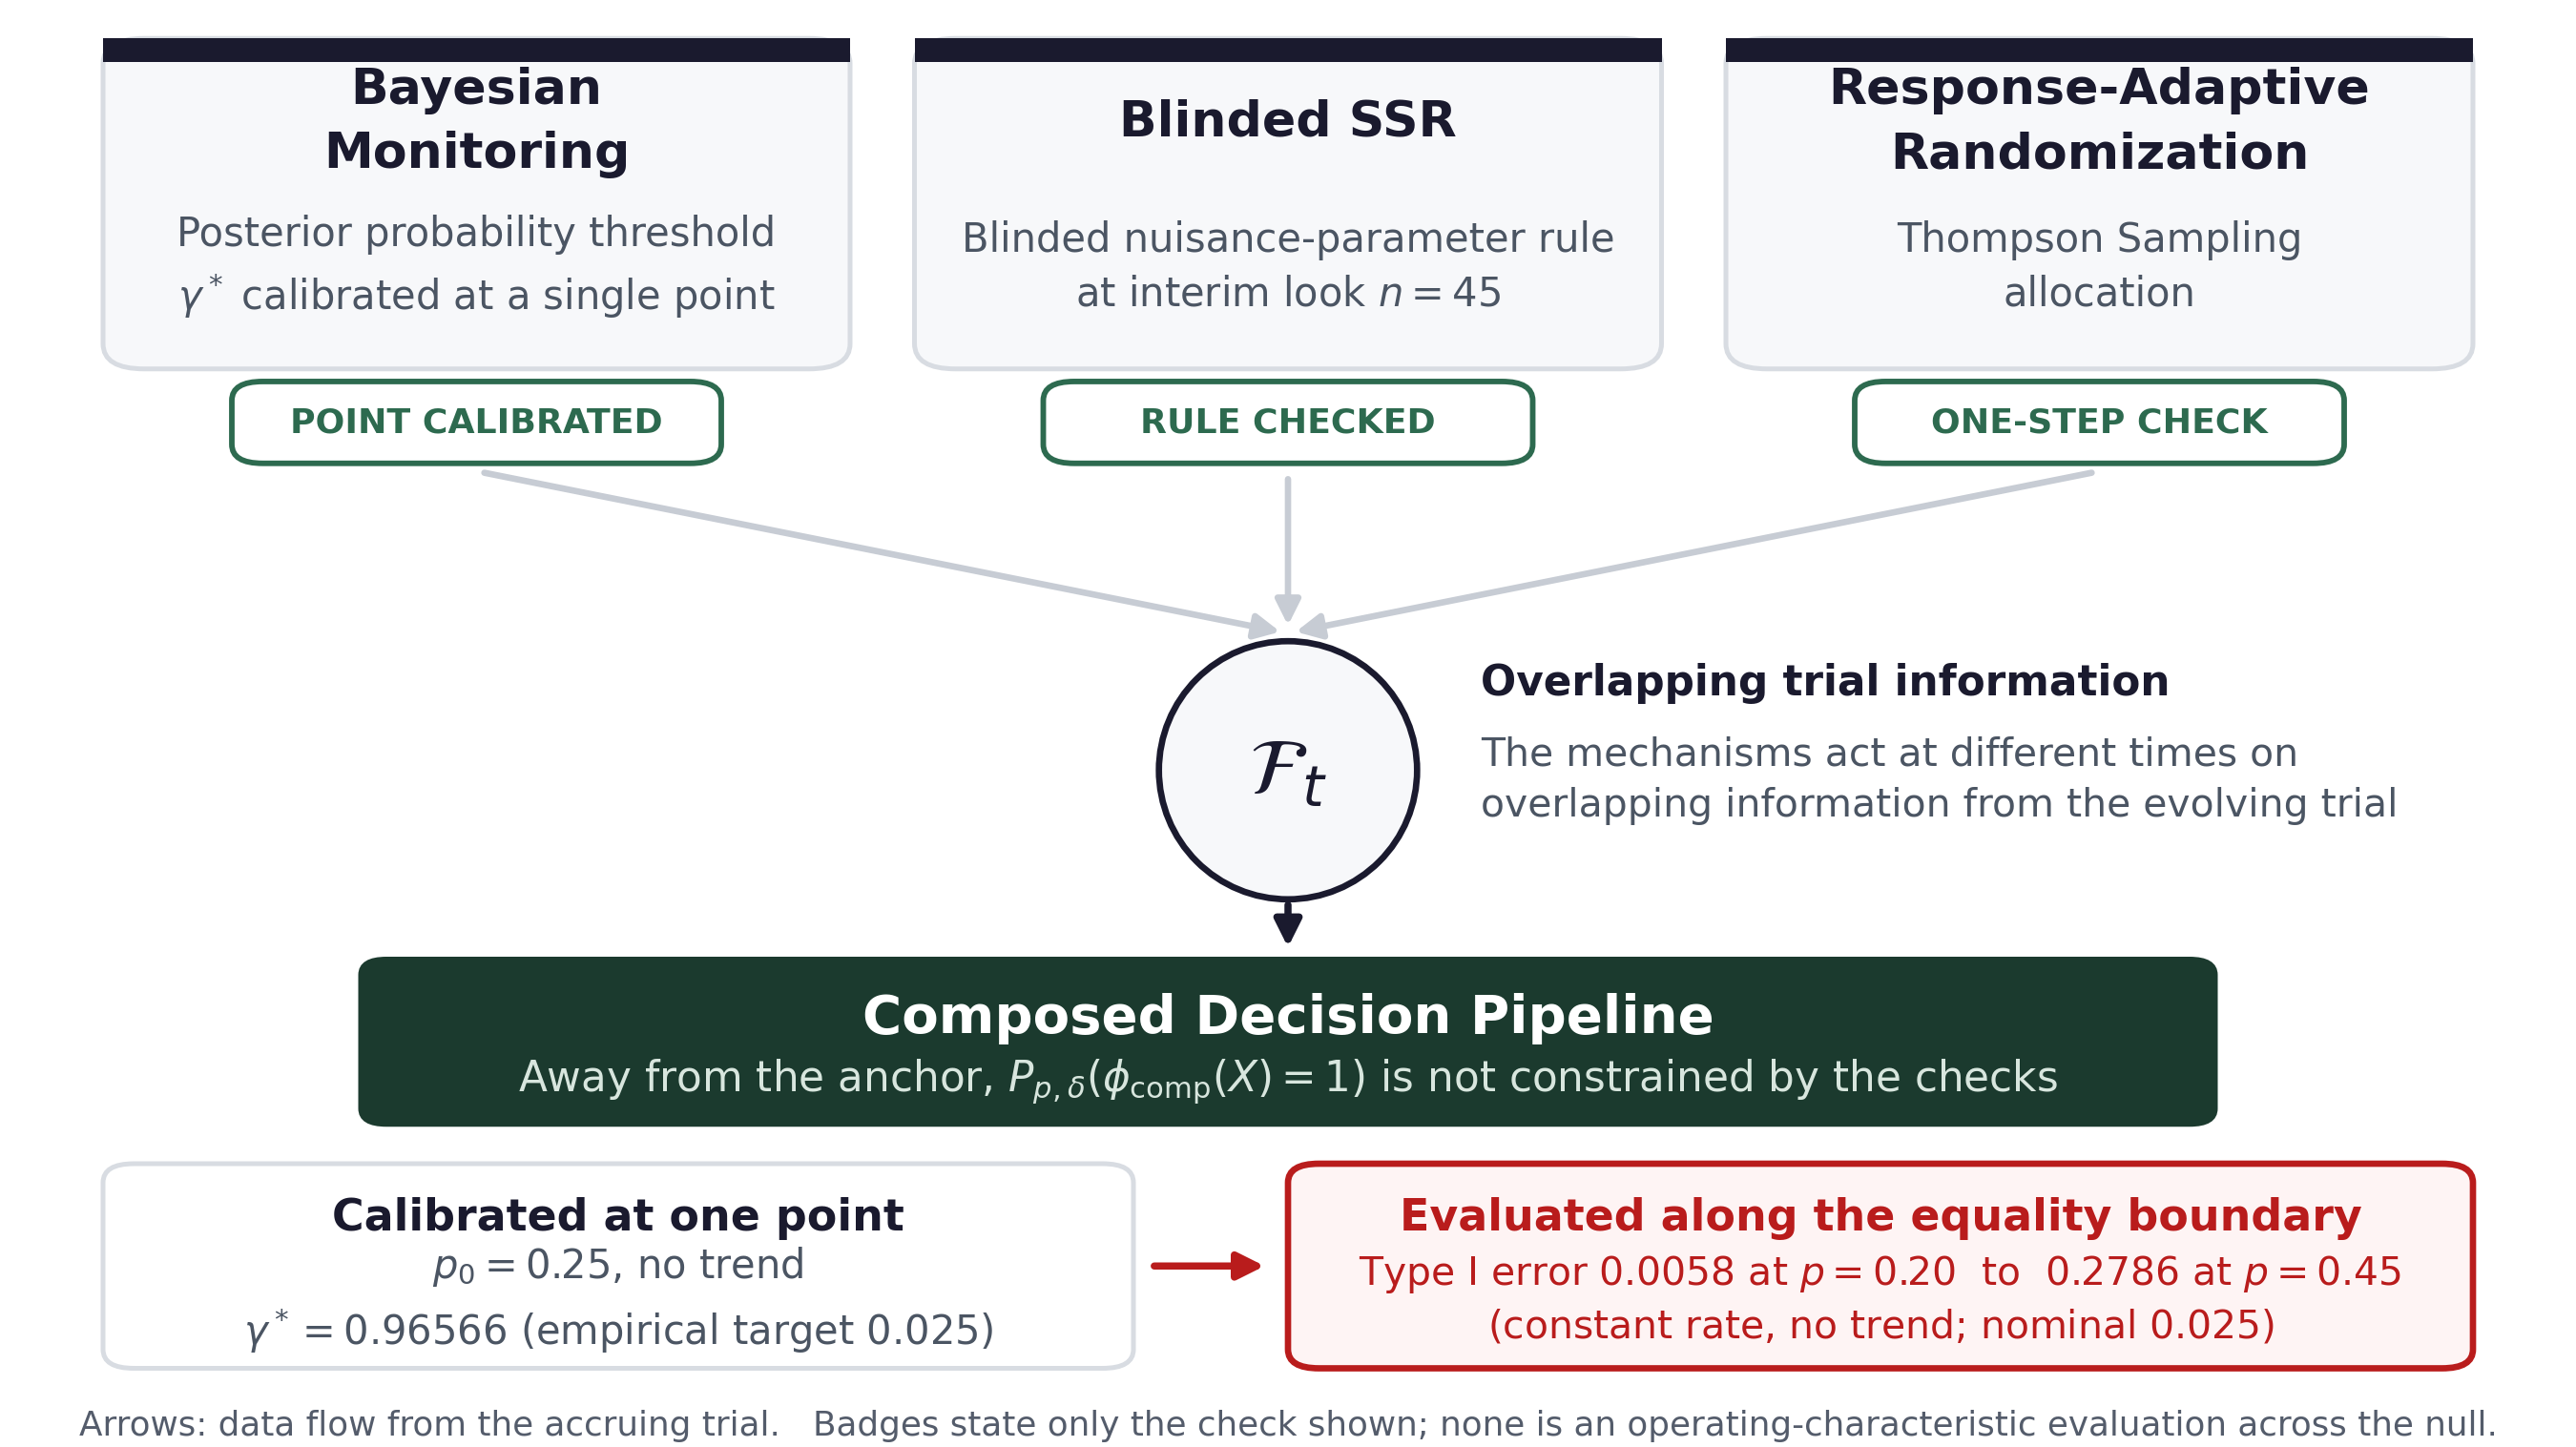
\includegraphics[width=\textwidth]{figures/Figure1_Composed_Design.png}
  \caption{Composed adaptive design: Bayesian monitoring, blinded
  nuisance-parameter SSR and RAR act at different times on overlapping
  information from the evolving trial---patient by patient, once at $n=45$ on
  blinded pooled counts, and at the scheduled looks respectively.  Component
  checks and point calibration at the anchor do not bound Type~I error
  elsewhere in the null.  The grid evaluated here is the equality boundary
  $p_e=p_c$, not the full composite null.}
  \label{fig:composed}
\end{figure}


% ─────────────────────────────────────────────────────────────────────────────
\section{Simulation Study}

\subsection{Design Specification}
\label{sec:design}

We simulate a two-arm Phase~II oncology design with MAP borrowing on the
control arm \citep{weber_rbest}, interim looks at $n=30,45,60$ and a final at
$n\geq90$ (post-SSR).  RBesT fits the historical cohorts ($n=50,40,60$;
38/150 responses) as a robustified mixture with components
\[
\begin{aligned}
&0.5887\,\mathrm{Beta}(18.403,53.273),\\[-2pt]
&0.2113\,\mathrm{Beta}(1.956,4.703),\quad\text{and}\quad
0.2000\,\mathrm{Beta}(1,1).
\end{aligned}
\]
The experimental-arm monitoring prior is $\mathrm{Beta}(0.5,0.5)$.  RAR
maintains separate $\mathrm{Beta}(0.5,0.5)$ posteriors for the two arms,
alternates allocation for a 10-patient burn-in, and thereafter assigns the
experimental arm when an independent draw from its posterior exceeds the
corresponding control-arm draw.
At 50\% enrollment, Rule~B uses only the pooled response count to estimate the
overall event-rate nuisance parameter, while the planned treatment effect
$\Delta=0.45-0.25=0.20$ remains fixed.  Under a prespecified working 1:1
allocation, it preserves the fixed-sample Wald power implied by the original
$N=90$ design (0.5296), permits increases only, and applies the protocol cap
$N=150$.  The working rates are
\[
\hat p_c=\operatorname{clamp}_{[10^{-6},\,1-\Delta-10^{-6}]}
(\hat p_{\rm pool}-\Delta/2), \qquad
\hat p_e=\hat p_c+\Delta.
\]
The recalculated per-arm size is
\[
 n_{\rm arm}=\frac{(z_{1-\alpha}+z_{\rm power})^2
 [\hat p_c(1-\hat p_c)+\hat p_e(1-\hat p_e)]}{\Delta^2},
\]
rounded up and doubled.  This pooled-data construction follows the blinded
binary internal-pilot principle of \citet{friede_kieser_2004}.  It is a
conventional-style working nuisance rule, not an exact power calculation for
the Thompson-sampling allocation or Bayesian final decision.  At the planned
$n=45$ look, its complete count mapping spans only $N=90$--100; the exact
expected $N$ is 90.44 at $p=0.25$, 91.57 at $p=0.30$, and 94.12 at $p=0.36$
under the active trend.  Thompson Sampling RAR is accompanied by a stand-alone
one-step check against analytical $P(\theta_e>\theta_c)$; that diagnostic does
not invoke the production allocation path in the trial simulator.

The threshold is calibrated at the design anchor $p_0=0.25$, distinct from the
dominant-component mean 0.2568, robustified-mixture mean 0.3132 and historical
pooled rate 0.2533.  We therefore describe $p>0.25$ only as departure from the
calibration anchor, not from the prior mean.

For enrollment position $i$, the response probabilities are
$p_e(i)=p_e+\delta(i-1)/89$ and $p_c(i)=p_c+\delta(i-1)/89$, with the evaluated
values inside $[0,1]$.  The superiority null is $H_0:p_e\leq p_c$.  The
constant-rate sweep evaluates its equality boundary, setting $p_e=p_c=p$ and
$\delta=0$.  A violation at any such point is sufficient to disprove uniform
control, but the sweep does not establish that the boundary is least favorable
or characterize the interior $p_e<p_c$.  The trend-active stress sweep also sets
the baseline rates $p_e=p_c=p$ and uses $\delta=0.05$, so
$p_e(i)=p_c(i)$ at every position while both drift; the analysis remains
time-constant.

The simulation completes enrollment to the total selected by Rule~B and then
evaluates the maximum posterior probability at total enrollments
$30,45,60,90$, plus the realised final sample size when it exceeds 90.
Because allocation,
outcomes and SSR do not depend on the efficacy boundary, thresholding this
maximum preserves the efficacy-only reject/no-reject indicator that prospective
monitoring with immediate outcomes would produce.  It does not simulate
operational early stopping and therefore does not estimate efficacy stopping
times, early-stopped sample sizes, or allocations after first boundary crossing.

Under $H_0$ both arms share baseline rate $p$ and drift together, so there is
no contemporaneous treatment effect; but the analysis is time-constant while the
data drift, so these quantities are kept outside the paper's constant-rate
Type~I error estimand and reported as rejection probabilities.  Within the wider $p=0.20$--$0.45$ trend grid,
we highlight $p=0.27$ and $p=0.30$ with linear trend $\delta=0.05$ over the
planned enrollment horizon.  These are sensitivity scenarios, not an asserted
empirical range; \citet{tang_2010} and
\citet{viele_2014} provide clinical and historical-borrowing context.

All primary Rule~B estimates carry binomial MCSE
$\sqrt{\hat p(1-\hat p)/N_{\rm sim}}$; cell-specific MCSEs and 95\% simulation
intervals are reported here or in the simulation supplement.  Downstream MCSEs
and intervals condition on the selected $\gamma^*$ and do not propagate its
calibration-sample uncertainty; the separate bootstrap below describes
threshold-selection variability only.

\textit{Note on calibration:} The efficacy threshold is obtained by grid-free
binary search, giving $\gamma^* = 0.96566$ with in-sample T1E $= 0.0248$
($N = 20{,}000$) at the design anchor $p_0 = 0.25$ with no trend.  No MCSE is
quoted for that value: $\gamma^*$ is chosen by bisection on this same sample,
so the achieved level is near-deterministic by construction.  The calibration
bootstrap gives $\gamma^*$ standard deviation 0.00106, 95\% interval
$[0.96303, 0.96759]$ over 500 resamples.
On an independent fresh-seed sample ($N=5{,}000$), T1E was 0.0224 (MCSE
0.0021; 95\% simulation interval $[0.0183,0.0265]$), compatible with the
nominal target.  Binary search still targets an empirical sample rather than
the population error rate, so neither estimate is exact calibration.


\subsection{Component-Level Numerical Checks}

Four isolated calculations were checked.  MAP prior: maximum deviation from
the RBesT mixture = $1.78 \times 10^{-15}$ (floating-point precision).  Both
sides of that comparison are computed from the same fitted mixture, so it is an
internal consistency check on the fitted object, not an external benchmark.
Posterior probabilities use deterministic 400-node Gauss--Legendre quadrature.
A targeted comparison of 12 representative reachable states nearest
$\gamma^*$ against adaptive integration found maximum deviation
$3.83\times10^{-12}$ and no decision flips; this was a targeted boundary check,
not an exhaustive enumeration.
Rule~B SSR: the calculation reproduces $N=90$ at the exact planning nuisance
rate, uses only the pooled interim count, is increase-only, returns even sample
sizes, and stays within the prespecified bounds; its full $n=45$ input support
was exhaustively checked.  The pooled nuisance construction is compared with
the framework of \citet{friede_kieser_2004}, but the embedded working Wald rule
is not claimed to reproduce the operating characteristics of their final test.
RAR one-step allocation: a stand-alone diagnostic has maximum deviation from
analytical $P(\theta_e > \theta_c)$ of 0.0036 (Monte Carlo error at
$n = 100{,}000$).  It reimplements one allocation draw and does not exercise
the production allocation path inside the trial simulator.  All four checks
pass their stated tolerances; none evaluates Type~I error away from the anchor.

\subsection{Constant-Rate Equality Boundary of the Composite Null}
\label{sec:constant-rate}

We first hold $\delta = 0$, so the response rate is constant over calendar time
and identical in both arms at every point of the grid.  Every point is then a
genuine null for the analysis actually performed, and every rejection is a
Type~I error in the conventional sense.  This isolates the robustness question
from any question about model misspecification.

\begin{center}
\begin{tabular}{ccccc}
\toprule
$p$ & SSR + RAR disabled & All mechanisms & MCSE (full) & Fixed-$\gamma^*$ difference \\
\midrule
0.20 & 0.0298 & 0.0058 & 0.0011 & $-0.0240$ \\
0.22 & 0.0356 & 0.0090 & 0.0013 & $-0.0266$ \\
0.25 & 0.0534 & 0.0236 & 0.0021 & $-0.0298$ \\
0.27 & 0.0780 & 0.0380 & 0.0027 & $-0.0400$ \\
0.30 & 0.0936 & 0.0810 & 0.0039 & $-0.0126$ \\
0.33 & 0.1330 & 0.1314 & 0.0048 & $-0.0016$ \\
0.36 & 0.1562 & 0.1854 & 0.0055 & $+0.0292$ \\
0.40 & 0.1778 & 0.2358 & 0.0060 & $+0.0580$ \\
0.45 & 0.2020 & 0.2786 & 0.0063 & $+0.0766$ \\
\bottomrule
\end{tabular}
\end{center}

\smallskip
At the calibration anchor $p=0.25$ the full design attains 0.0236
(MCSE 0.0021), consistent with the nominal 0.025.  The estimated Type~I error
increased at every successive evaluated grid point: 0.0380 at $p=0.27$, 0.0810 at $p=0.30$, 0.1854 at
$p=0.36$ and 0.2786 at $p=0.45$.  \textbf{Calibration at a point does not
deliver control over the composite null, and no calendar trend or
time-model misspecification is needed to show it.}

The two largest rates characterise the shape of the curve; we do not assert
that they are plausible control rates for this indication.  We note also that
$p=0.45$ is a \emph{null} scenario in which
both arms sit at 0.45, so there is no treatment effect; the value is
numerically equal to the experimental-arm rate assumed under the planning
alternative (against a 0.25 control), but the coincidence is arithmetic only
and that row is not an alternative-hypothesis evaluation.
Over the lower evaluated range $p=0.27$--$0.36$---departures of two to eleven
percentage points from the anchor---Type~I error runs from 0.0380 to 0.1854,
up to 7.4 times nominal.

\subsection{Trend-Active Stress Analysis}
\label{sec:trend-active}

We next activate a shared calendar trend in both arms while retaining the
time-constant analysis.  Contemporaneously there is still no treatment effect,
but the analysis is misspecified for the time-varying data-generating process.
We therefore report both columns as rejection probabilities rather than Type~I
errors for the constant marginal-rate null.  This caution applies even when RAR
is disabled.  The implemented rule, ${\tt arm}=(i-1)\bmod 2$, gives
deterministic strict alternation: control occupies odd enrollment positions and
experimental treatment occupies even positions.  By construction, this balances
counts at even looks and tightly interleaves enrollment time, but it is not exact
time balance under the coded patient-level trend.  At every even look, experimental patients
are one position later within each pair, so their average generating rate
exceeds control by $\delta/(N_{\mathrm{base}}-1)=0.05/89\approx0.00056$; at the
odd $n=45$ look, arm counts differ by one.  With RAR active the allocation
additionally depends on accumulating data.  This study does not identify a
time-adjusted estimand or measure either allocation--time mechanism.

\begin{center}
\begin{tabular}{cccc}
\toprule
$p$ & SSR + RAR disabled & All mechanisms & Fixed-$\gamma^*$ difference \\
\midrule
0.20 & 0.0342 & 0.0092 & $-0.0250$ \\
0.22 & 0.0474 & 0.0208 & $-0.0266$ \\
0.25 & 0.0742 & 0.0484 & $-0.0258$ \\
0.27 & 0.0900 & 0.0754 & $-0.0146$ \\
0.30 & 0.1180 & 0.1206 & $+0.0026$ \\
0.33 & 0.1398 & 0.1670 & $+0.0272$ \\
0.36 & 0.1644 & 0.2286 & $+0.0642$ \\
0.40 & 0.1894 & 0.2798 & $+0.0904$ \\
0.45 & 0.1970 & 0.2874 & $+0.0904$ \\
\bottomrule
\end{tabular}
\end{center}

\smallskip
Two readings follow.  First, \textbf{at the full-design threshold, disabling
SSR and RAR does not return the rejection probability to the nominal level}:
with both switched off, it still rises from 0.0342 at $p = 0.20$ to 0.1970 at
$p = 0.45$.
That column is the same fixed-threshold ablation used throughout
(Section~\ref{sec:factorial})---it carries $\gamma^*$, which was calibrated
with SSR and RAR active.  At $p=0.25$ on this trend-active slice it is 0.0742;
neither that row nor the full-design row is the no-trend calibration scenario.
Read it as ``the design with the adaptive components switched off, threshold
unchanged'', not as a calibrated monitoring-only design.  Second,
\textbf{at fixed $\gamma^*$, enabling SSR and RAR lowers the rejection
probability at low $p$ and raises it at high $p$}: the difference runs from
$-0.0250$ at $p = 0.20$ to $+0.0904$ at $p = 0.45$, reversing sign across the
range.

The grid establishes a direction change, not its crossing point: the contrast
at $p=0.30$ is $+0.0026$ against a Monte Carlo standard error of 0.0065, and
the neighbouring rates are 0.27 and 0.33.  It also shows elevated rejection
probabilities across the grid but does not locate their supremum.  The largest
\emph{estimated}
rejection probability on this grid is 0.2874; that is a Monte Carlo estimate
carrying an MCSE of 0.0064, not a deterministic bound, and a one-sided 95\%
simulation limit places that rate's rejection probability at or above 0.2769.

Comparing this grid with the constant-rate grid of
Section~\ref{sec:constant-rate} at matched baseline rates, the trend's
contribution is \emph{not} monotone in the departure.  The trend-active point
estimate is higher throughout: the difference rises from $+0.0034$ at
$p=0.20$ to $+0.0396$ at $p=0.30$, dips to $+0.0356$ at $p=0.33$, reaches
$+0.0440$ at $p=0.40$, and falls to $+0.0088$ at $p=0.45$.  The first gap is
borderline (2.0 Monte Carlo standard errors) and the last is indistinguishable
from zero (1.0 standard error), so no uniform separation is claimed.  The fall
from $p=0.40$ to $p=0.45$ is $-0.0352$, about 2.8 standard errors, and rests on
one point at the grid boundary.  We report it as an observation about that point
and offer no mechanism.  The more aggressive Rule~A stress test is summarized in
Appendix~\ref{app:rule-a}.

% Figure 2 belongs to this section; [htb] let it drift past the next heading
% and land after the 3.6 table. [t!] plus a \FloatBarrier after it keeps the
% figure with the text that discusses it.
\begin{figure}[t!]
  \centering
  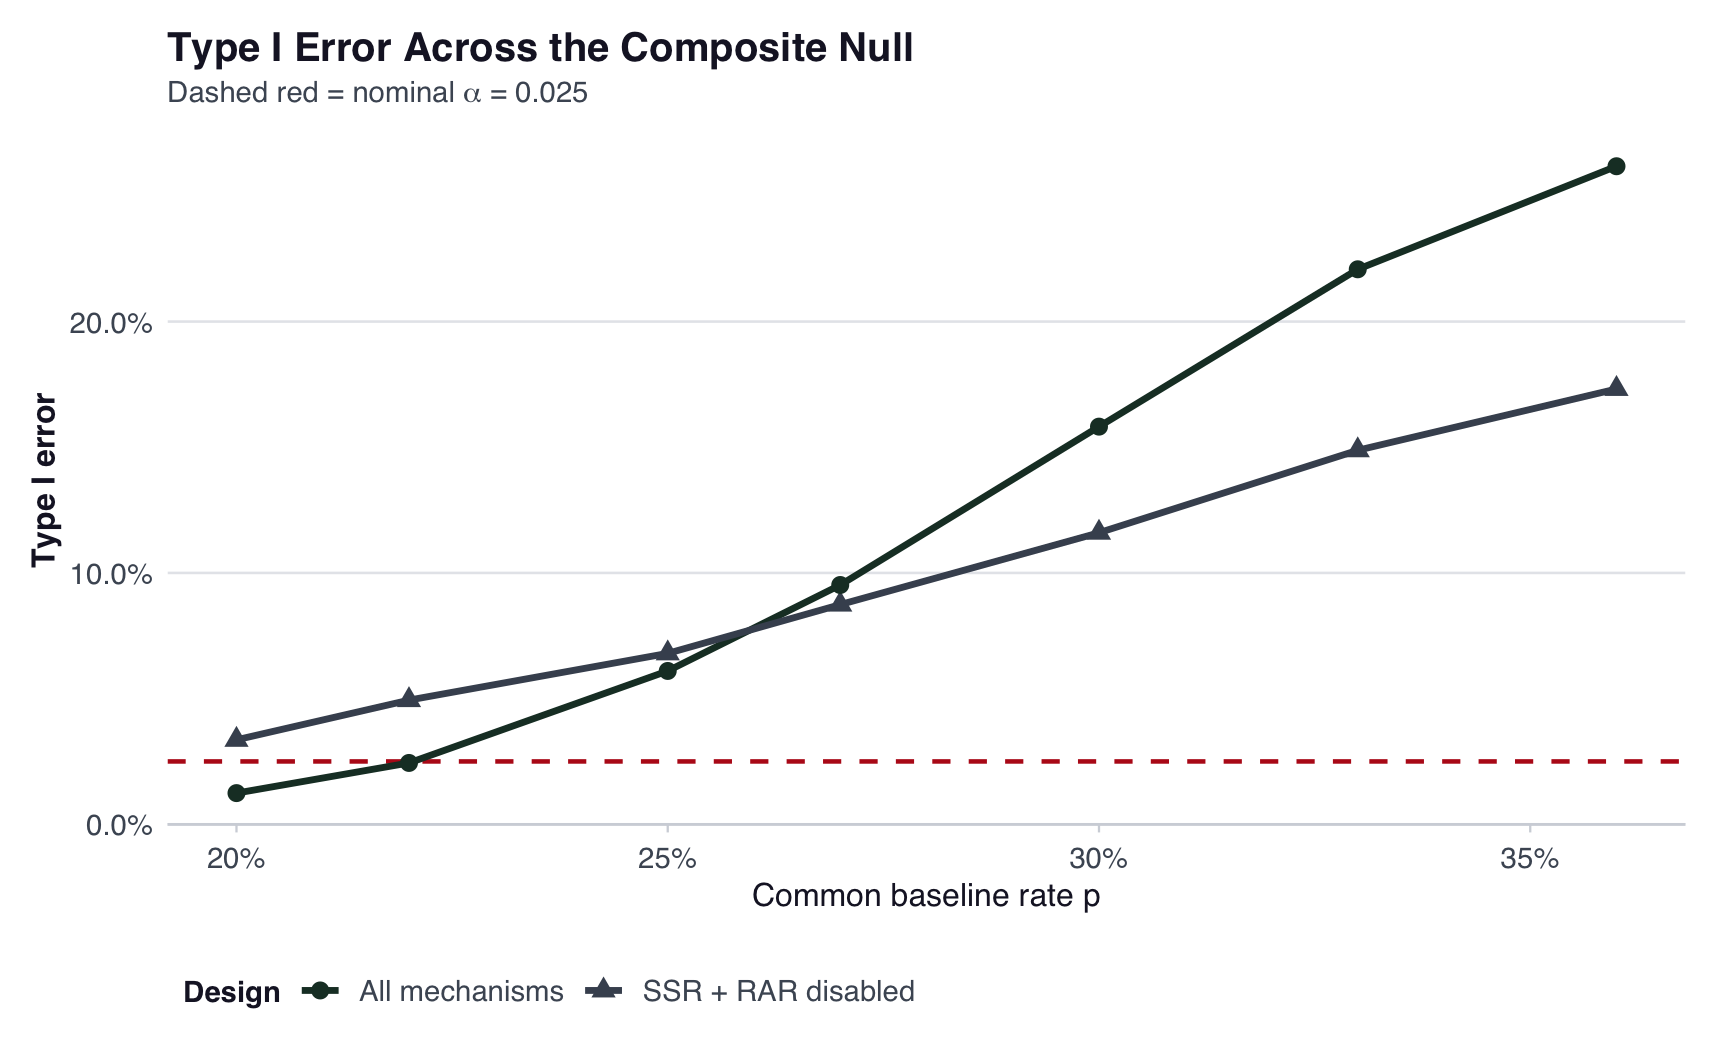
\includegraphics[width=0.86\textwidth]{figures/composite-null-plot-1.png}
  \caption{Rejection probability across the common-rate grid.  \textbf{Left
  panel:} the constant-rate equality boundary of the superiority null
  ($\delta=0$), where the time-constant likelihood matches the data-generating
  process and every rejection is a Type~I error.  \textbf{Right
  panel:} the trend-active stress scenario ($\delta=0.05$), where both arms
  drift together but the analysis remains time-constant; those rejections are
  kept outside the constant-rate Type~I error estimand and are reported as
  rejection probabilities.  In
  both panels, grey holds the full-design threshold with SSR and RAR disabled
  and dark green shows all mechanisms; both are fixed-threshold comparisons,
  not separately calibrated designs.  Dashed red line: nominal
  $\alpha=0.025$.}
  \label{fig:composite}
\end{figure}
\FloatBarrier


\subsection{Fixed-Threshold Factorial Ablation: SSR by RAR}
\label{sec:factorial}

Four designs (SSR $\times$ RAR), all at $p = 0.30$ with the trend active:

\begin{center}
\begin{tabular}{lcc}
\toprule
Condition & Rejection probability & MCSE \\
\midrule
SSR + RAR disabled       & 0.1120 & 0.0045 \\
$+$ SSR only             & 0.1248 & 0.0047 \\
$+$ RAR only             & 0.1236 & 0.0047 \\
$+$ SSR and RAR          & 0.1124 & 0.0045 \\
\bottomrule
\end{tabular}
\end{center}

\textit{These are ablations at a fixed threshold, not a decomposition.}
$\gamma^*$ was calibrated with SSR and RAR active; disabling components while
retaining it does not yield separately calibrated designs or attributable
shares.  The baseline cell is therefore not ``the excess caused by
monitoring'', although it does show that disabling both components leaves the
rejection probability far above the nominal level.  These cells are trend
active, so the quantity elevated here is a rejection probability, not a
Type~I error.

\textit{The SSR-enabled cells can accrue an additional efficacy analysis.}
The monitoring schedule is $\{30,45,60,90\}$ together with the realised final
sample size, so a trial that SSR extends beyond $N=90$ is analysed five times
while a fixed-$N$ trial is analysed four.  Because the test statistic is a
maximum over looks, the SSR-enabled cells receive one further opportunity to
cross the threshold in the $\Pr(N>90)$ fraction of replicates, which is 0.3157
at $p=0.30$.  This is correct trial conduct -- an extended trial does analyse
at its realised final $N$ -- but it means every full-design-versus-ablation
contrast reported here combines the adaptive mechanisms with a difference in
multiplicity, and no contrast should be read as isolating the mechanisms
alone.

The descriptive simple-contrast point estimates are
$\Delta_{\mathrm{SSR}\mid\mathrm{RAR}=0}=+0.0128$ and
$\Delta_{\mathrm{RAR}\mid\mathrm{SSR}=0}=+0.0116$; the combined
baseline-referenced contrast is $+0.0004$, with approximate Monte Carlo
standard errors 0.0063--0.0065.  The higher-precision replicate
($N=20{,}000$ per cell) estimates the same combined contrast at $+0.0092$, and
pooling the two gives $+0.0074$ (SE 0.0029, 95\% SI $[+0.0018,+0.0130]$), which
excludes zero.  We still draw no directional component conclusion, and the
reason is structural rather than a matter of precision: $\gamma^*$ was
calibrated once with every mechanism active and each ablation retains it, so
these cells are not separately calibrated designs and no contrast between them
partitions the excess.  More replicates would sharpen the contrast without
making it attributable.

The interaction was estimated on two disjoint seed blocks using the same
implementation.  The first run
($N=5{,}000$ per cell) gave $-0.0240$ (propagated MCSE 0.0091, 95\% SI
$[-0.0419,-0.0061]$), which excludes zero.  A higher-precision replicate on a
disjoint seed block ($N=20{,}000$ per cell) gave $-0.0037$ (MCSE 0.0046; 95\%
SI $[-0.0126,+0.0052]$), which does not.  The two are 2.0 standard errors apart
(heterogeneity $Q = 3.96$ on 1 df, $p = 0.047$) -- near the edge of what
independent sampling produces unaided, and not on its own evidence of a defect.
Their inverse-variance pooled estimate is $\Delta_\text{interaction} = -0.0077$
(SE 0.0041; 95\% SI $[-0.0157,+0.0002]$).

We report the pooled value and draw no directional conclusion.  The
lower-precision run's interval excluding zero is not reproduced by the
better-powered replicate, and we do not interpret it on its own.  Joint evaluation
remains necessary because an interaction is possible, but its sign and
magnitude should not be inferred from these runs.

\begin{figure}[htb]
  \centering
  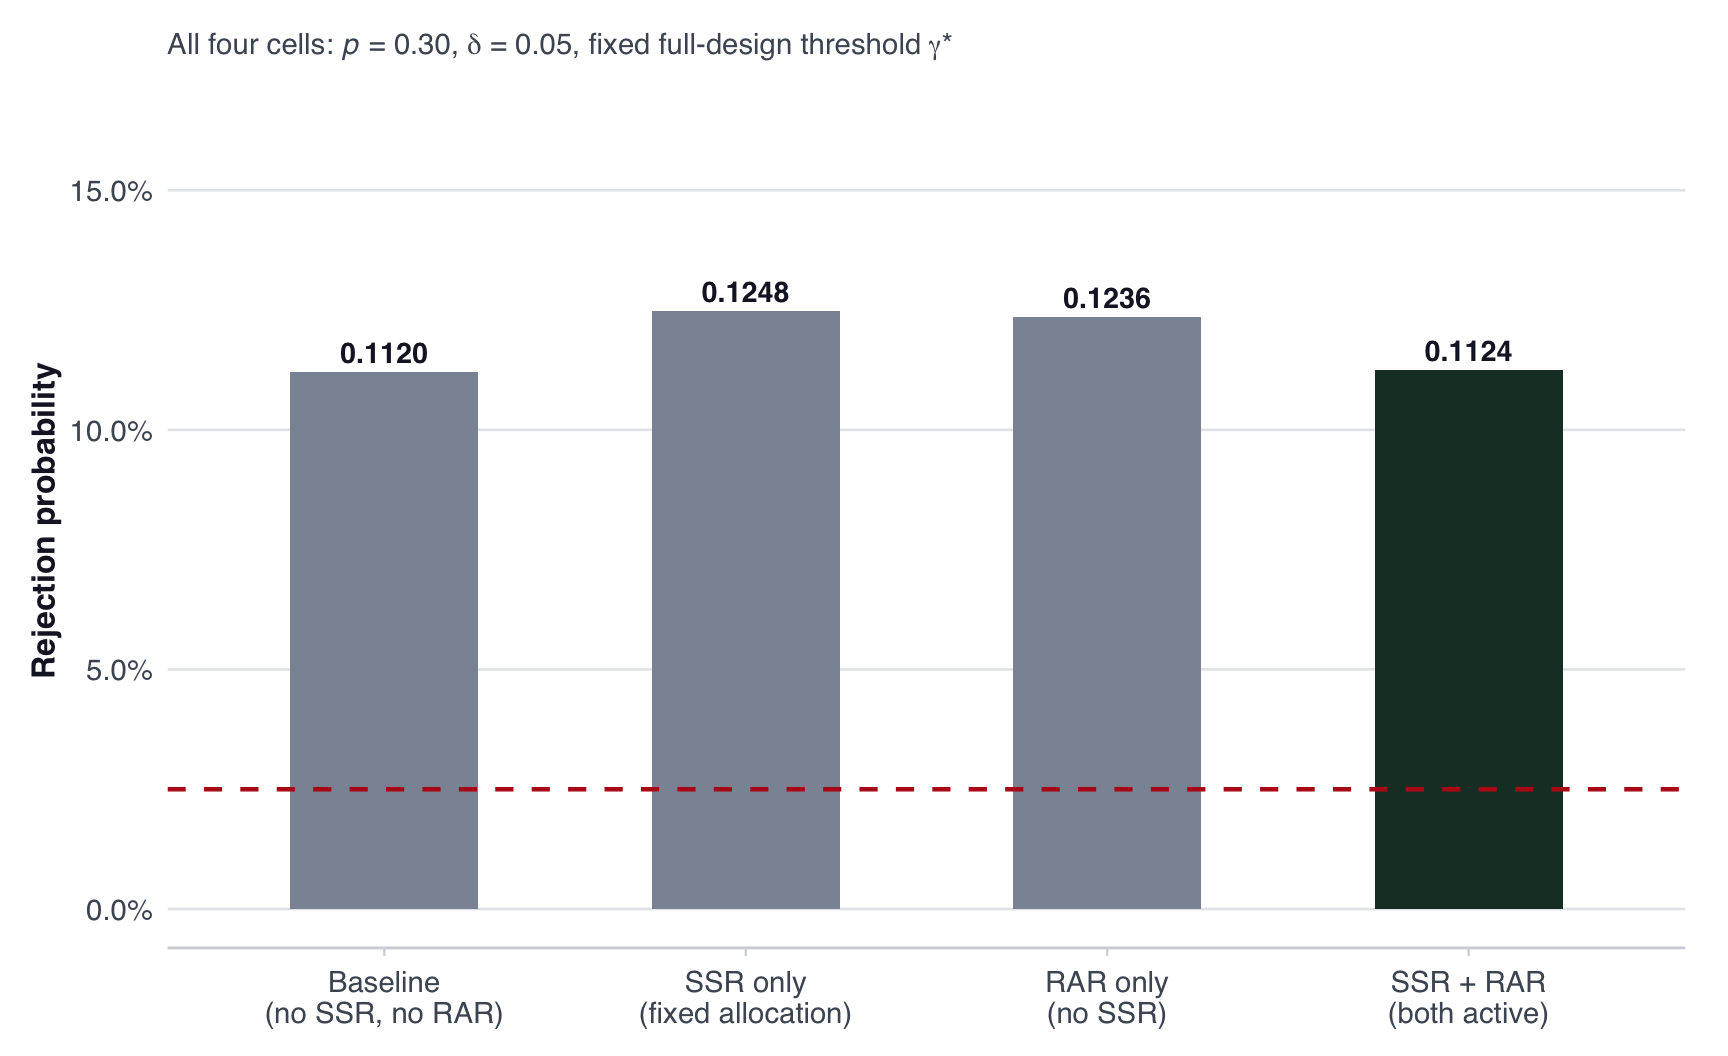
\includegraphics[width=0.86\textwidth]{figures/factorial-1.png}
  \caption{Fixed-threshold Rule~B factorial ablation of SSR by RAR at $p=0.30$
  with the shared trend active.  Simple contrasts
  $\Delta_{\mathrm{SSR}\mid\mathrm{RAR}=0}=+0.0128$ and
  $\Delta_{\mathrm{RAR}\mid\mathrm{SSR}=0}=+0.0116$.  The
  interaction is estimated on two disjoint seed blocks; the inverse-variance
  pooled estimate is
  $-0.0077$ (95\% SI $[-0.0157,+0.0002]$), which includes zero.  Bar labels are
  cell estimates; the interaction is not annotated in the panel because it is a
  four-cell contrast rather than a property of any one bar.  Dashed red line =
  nominal $\alpha=0.025$.}
  \label{fig:factorial}
\end{figure}

\subsection{Baseline-Rate Departure by Time Trend}
\label{sec:factors}

A 2$\times$2 factor crossing evaluates departure and trend under the primary
design; both factors feed monitoring, SSR and RAR, so it does not isolate those
channels.

\begin{center}
\begin{tabular}{lcc}
\toprule
Condition & Rejection probability & vs.\ anchor run \\
\midrule
Anchor, no trend (independent run) & 0.0232 & --- \\
Departure only & 0.0904 & $+0.0672$ \\
Trend only & 0.0474 & $+0.0242$ \\
Both & 0.1140 & $+0.0908$ \\
\midrule
Additive prediction & 0.1146 & \\
Interaction term & $-0.0006$ & \\
\bottomrule
\end{tabular}
\end{center}

The departure-only simple contrast is $+0.0672$, and the trend-only simple
contrast is $+0.0242$.  Because both factors feed monitoring, SSR and RAR,
neither contrast is attributable to a single channel.  Unlike the
fixed-threshold ablations, all four cells use the full design and the same
independently simulated anchor/no-trend reference condition.  The interaction
is $-0.0006$ (MCSE 0.0071; 95\% SI $[-0.0145,+0.0133]$).  Its point estimate is
consistent with additivity at these factor levels, while the interval allows
modest departures in either direction.  It is a risk-difference interaction at
these factor levels and includes the additional trend exposure from enrollment
beyond $N=90$; Rule~B limits that extension to 100 at the planned SSR look.

\begin{figure}[htb]
  \centering
  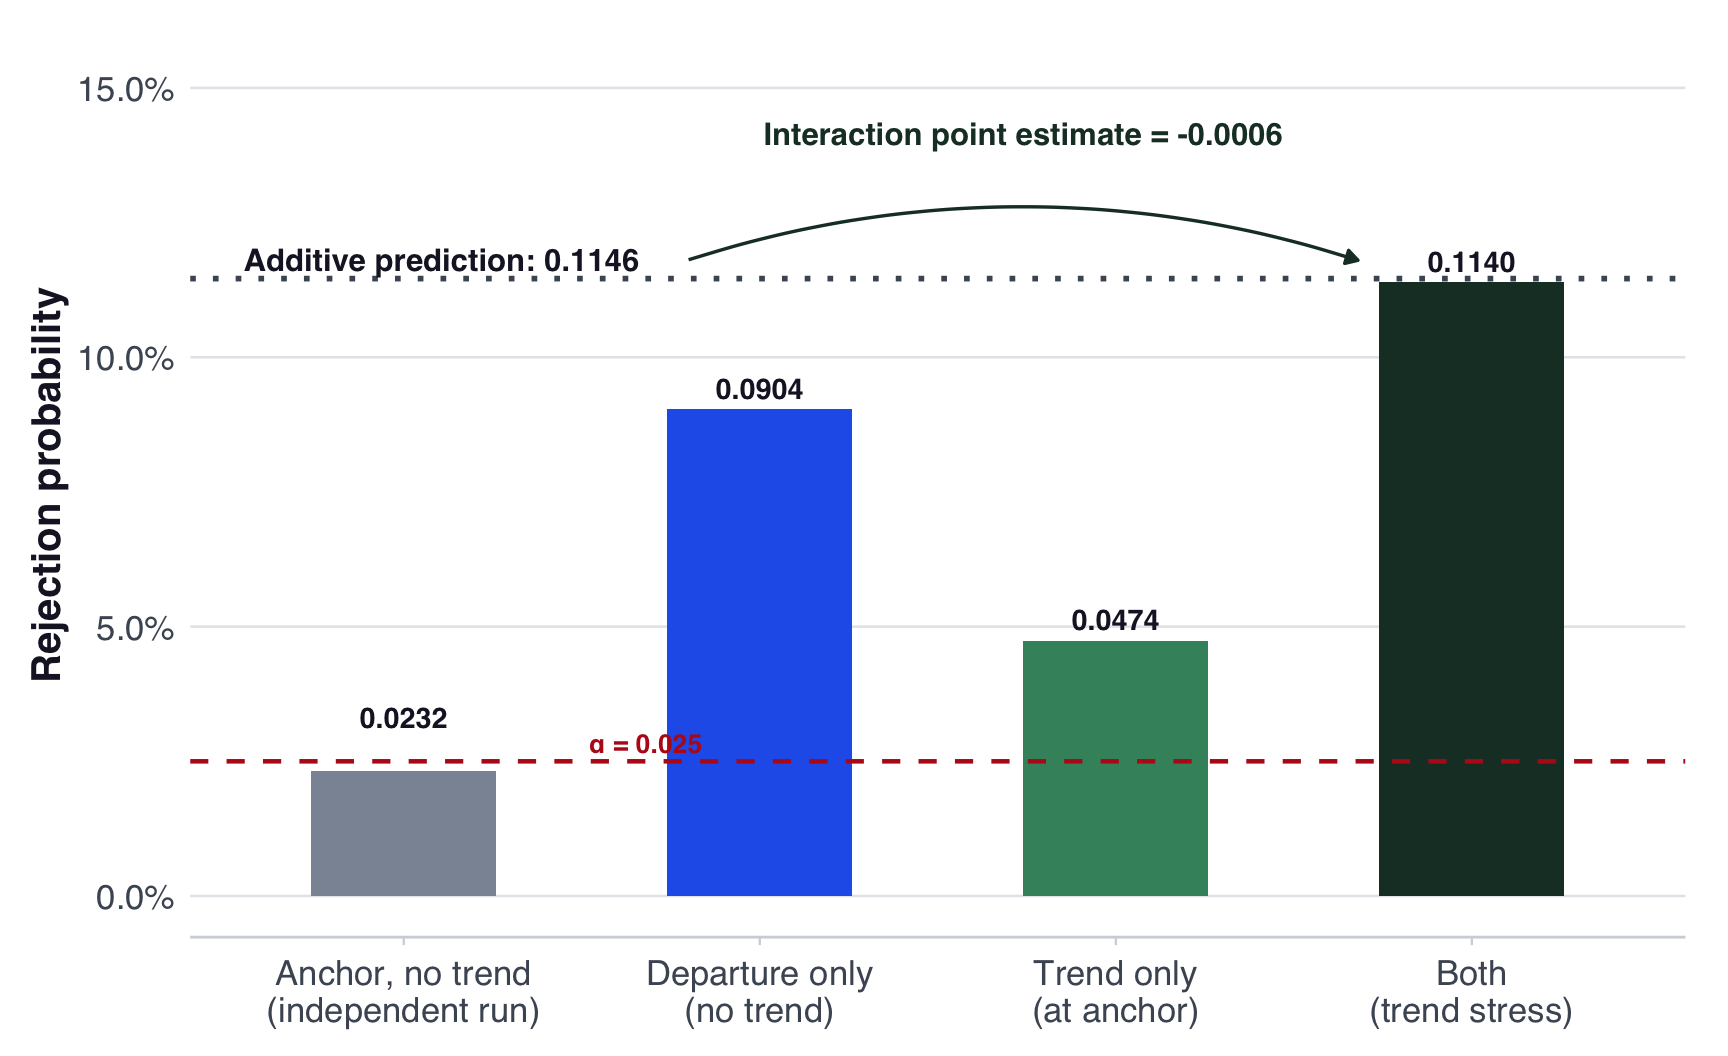
\includegraphics[width=0.86\textwidth]{figures/departure-trend-crossing-1.png}
  \caption{Departure-by-trend crossing under the full design.  The interaction
  is $-0.0006$ (95\% SI $[-0.0145,+0.0133]$); dashed red line denotes nominal
  $\alpha=0.025$.}
  \label{fig:factors}
\end{figure}

\subsection{Sensitivity Analyses}
\label{sec:sens}

The following sweeps use the five-percentage-point departure ($p = 0.30$) to
characterize mechanism sensitivity across a wider range.

\begin{itemize}[noitemsep]
  \item \textbf{Departure severity}, at constant trend
    ($p \in \{0.25, 0.27, 0.30\}$, all with $\delta = 0.05$): the rejection
    probability increases monotonically, 0.0484 $\to$ 0.0754 $\to$ 0.1206,
    with no direction reversal.
  \item \textbf{Vague-component weight} (0--90\%): larger weight on the flat
    robustify component means less borrowing; the rejection probability
    declines from 0.1488 to 0.0624.
  \item \textbf{Time trend} $\delta$ (0--15\%): the rejection probability
    increases from 0.0812 at $\delta=0$---which is a Type~I error, the trend
    being absent---to 0.2220 at $\delta=0.15$.
  \item \textbf{SSR trigger timing}: moving the primary look from $n=45$ to
    $n=30$ changed the rejection probability from 0.1161 to 0.1244; a separate
    sweep over
    $n_\text{SSR}\in\{20,30,40,45,55,60\}$ ranged from 0.1126 to 0.1234.
    Timing also changes the realised final-$N$ distribution, so these are not
    isolated timing effects.
\end{itemize}

% ─────────────────────────────────────────────────────────────────────────────
\section{Discussion}

\subsection{Regulatory Implications and Recommendations}

An efficacy threshold calibrated at one assumed control rate need not control
Type~I error elsewhere in the composite null.  The FDA January 2026 draft
guidance recommends comprehensive simulation over plausible assumptions and
asks sponsors to discuss the handling of prior--data conflict.  We go further,
on the strength of the results above: operating-characteristic evaluation
should span a prespecified set of null-generating conditions, and the handling
of prior--data conflict should be prespecified rather than discussed post hoc.
That extension is ours, not the guidance's.

For designs of the kind studied here---binary endpoint, MAP borrowing on the
control arm, and a threshold calibrated at a single assumed control
rate---sponsors should (1) evaluate a grid of plausible control
rates rather than one anchor; (2) label whether component ablations are
separately calibrated, since a fixed-threshold ablation tests restoration of
control rather than attribution; and (3) cross departure and time trend rather
than rely only on separate one-factor analyses.

\subsection{Mitigation Strategies}
\label{sec:mitigation}

Potential safeguards include more robust or dynamic borrowing, pre-specified
prior--data disagreement diagnostics, pipeline-level recalibration of
$\gamma^*$ over the null grid, and an explicit maximum acceptable T1E over a
stated robustness range.  Each changes the composed pipeline and must itself be
evaluated at pipeline level; no component-level argument guarantees restored
control.

\subsection{Limitations and Future Work}

This paper demonstrates a control failure by simulation in one specific
design.  We did not evaluate other borrowing methods, endpoints, sample sizes
or $\alpha$ levels, and the recommendations above are offered as reasonable
practice rather than as results.  Several further limitations bound what is
established here.

\emph{The supremum is not estimated.}  The grid exhibits points at which
control fails.  The largest \emph{estimated} Type~I error on the constant-rate
grid is 0.2786, which is a Monte Carlo estimate with an MCSE of 0.0063 and may
lie either side of the true value at that rate; a one-sided 95\% simulation
limit places the Type~I error at $p=0.45$ at or above 0.2682.  Because the
supremum is at least the value at every evaluated point, the same pointwise
limit is also a lower confidence bound for the supremum---conditional on the
selected $\gamma^*$.  Its 95\% coverage is with respect to Monte Carlo error at
that rate only; it does not propagate the calibration-sample uncertainty in the
threshold (bootstrap SD 0.00106), and is therefore not an unconditional
statement.  Neither
figure locates the worst case, and
the curve has not flattened at the grid boundary.  The final three increments
are $+0.0540$, $+0.0504$ and $+0.0428$, but they span unequal steps in $p$
($0.03$, $0.04$, $0.05$); per percentage point of $p$ the increase is
$0.0180$, $0.0126$ and $0.0086$, so the series is decelerating while still
rising.  The supremum over
the composite null is therefore not located, and may lie above any value
evaluated here.  Locating the supremum, estimating it sharply, or constructing
an upper confidence bound would require a search beyond this finite grid.

\emph{Composition is not established as the cause.}  The title and
Section~\ref{sec:composed-defn} describe the setting: a design in which several
adaptive mechanisms act on overlapping information.  The study does not show
that composition produced the failure.  It cannot: $\gamma^*$ is calibrated once
with all mechanisms active and every ablation retains that threshold, so the
ablation rows answer whether switching a mechanism off restores control, not
whether composition caused the loss.  Answering the causal question would
require separately calibrated designs at each configuration, which we did not
run.  Relatedly, we evaluated no zero-borrowing condition---the vague-component
sweep reaches 90\% weight, not 100\%---so the contribution of MAP borrowing
cannot be separated from that of monitoring and adaptation.

\emph{No power evaluation is reported for the composed design.}  The only power
figure here is the 0.5296 fixed-sample Wald reference implied by $N=90$.  The
safeguards in Section~\ref{sec:mitigation} would each change the operating
characteristics, and recalibrating $\gamma^*$ over a null grid would raise the
threshold and cost power; we did not quantify that cost.  None of the
safeguards was simulated.  They are hypotheses about what would restore
control, not results.

\emph{Only the equality boundary is evaluated.}  The constant-rate grid covers
$p_e=p_c=p$, a one-dimensional boundary slice of $H_0:p_e\leq p_c$.  Failure at
any one of those points is enough to refute uniform control, but the simulations
do not establish the least-favorable configuration or characterize the interior
$p_e<p_c$.

\emph{Conflict is not quantified.}  We vary the calibration-anchor departure,
not a prior-predictive conflict measure.  Extending prior--data diagnostics such
as \citet{matthews_qian_fms,qian_matthews_fms_ops} from Normal-mean settings to
this binary MAP-mixture design would require a new statistic and calibration.

\emph{Rule~B is a working nuisance calculation, not exact design power.}  Its
1:1 Wald model differs from the RAR allocation and Bayesian final decision; the
0.5296 reference power and 90--100 mapping follow from the original $N=90$
design.  Results are conditional on this prespecified rule.  Appendix~\ref{app:rule-a}
summarizes the more aggressive Rule~A stress test.

\emph{No sufficient condition is proved.}  Shared information neither
guarantees nor precludes error control; a conditional-error or design-specific
argument would be required.

\emph{Calibration is Monte Carlo.}  Binary search targets the empirical
calibration sample; a fresh-seed validation was compatible with nominal, but
neither finite simulation establishes the population error rate exactly.

\emph{Numerical integration is implementation-specific.}  Posterior
probabilities use the stated 400-node Gauss--Legendre rule.  The 12-state
near-boundary comparison found no decision flips, but it was not an exhaustive
audit of all reachable states and does not establish invariance to a different
integration rule.  The reported operating characteristics are conditional on
this implementation.

\emph{The implementation is efficacy-only.}  Retrospective evaluation of the
maximum posterior probability preserves the reject/no-reject indicator because
the boundary does not drive allocation, outcomes or SSR, but it does not
reproduce operational early stopping or estimate stopping-time and post-stop
quantities.

\emph{Outcome timing and accrual are simplified.}  Outcomes are available
immediately for per-patient RAR updates, and enrollment index is used as a proxy
for calendar time.  Delayed outcome availability and stochastic accrual are not
modeled.

\emph{Component ablations are not separately calibrated.}  They retain the
full-design $\gamma^*$ and answer whether disabling a component restores
control, not how much excess it caused.  Attribution would require calibrating
each design separately.

% ─────────────────────────────────────────────────────────────────────────────
\section{Conclusion}

Point calibration did not provide uniform Type~I error control across the
composite null.  At the full-design threshold, disabling SSR and RAR did not
restore it on the constant-rate grid.  The fixed-$\gamma^*$ contrast reversed sign across the
evaluated null rates, but the Rule~B factorial and departure-by-trend
interaction intervals both included zero; the simulations do not support a
stable interaction claim in either direction.

The practical consequence is a reporting standard rather than a new method.
Operating characteristics should be evaluated over a prespecified grid of
null-generating conditions.  Fixed-threshold ablations can show whether
disabling a component restores control, but attribution requires separately
calibrating each design.  The simulation code is publicly available for
independent verification and extension; the Zetyra platform is a commercial
SaaS product.

\medskip\noindent\textit{Calibrate at a point.  Validate over the null.}

% ─────────────────────────────────────────────────────────────────────────────
\section*{Acknowledgements}

Simulation source, manuscript source, figures and reproducibility instructions:\\
\href{https://github.com/evidenceinthewild/Composed-Adaptive-Trial-Validation}{github.com/evidenceinthewild/Composed-Adaptive-Trial-Validation}.
Rule~A is summarized in Appendix~\ref{app:rule-a} as a method-development
stress test, not as the primary analysis.

% ─────────────────────────────────────────────────────────────────────────────
\appendix
\section{Original Rule A Pooled Conditional-Power Stress Test}
\label{app:rule-a}

The original Rule~A treated the pooled interim rate as a one-sample signal
against $p_0=0.25$ and increased total sample size to target 80\% conditional
power, capped at $N=150$.  A common upward nuisance shift under the two-arm null
could therefore drive expansion, so it was replaced before publication by
Rule~B.  With $\gamma^*=0.96596$, Rule~A reached a higher rejection
probability at $p=0.36$ under the trend-active null grid than Rule~B's 0.2286
at the same rate.  We give no figure for it: the Rule~A run is not part of the
primary release, and its simulation budget and Monte Carlo standard error are
not reported here, so a four-decimal value would carry an authority nothing
released can support.  The comparison is retained only to record why Rule~A was
replaced.

% ─────────────────────────────────────────────────────────────────────────────
% Tighten the reference list: natbib's default inter-entry spacing pushed
% two entries onto a page of their own.
\setlength{\bibsep}{0.6ex plus 0.2ex}
\bibliographystyle{plainnat}
\bibliography{references}

\end{document}
